\documentclass[french,oneside]{wfrp}

% No indent length document-wise.
\setlength\parindent{0pt}

\usepackage[hidelinks,frenchlinks=true]{hyperref}

\begin{document}

\chapter{La peste de Karlsheim}
\label{chap:la-peste-de-karlsheim}

\section{Contexte}
\label{sec:contexte}

L’aventure se déroule en l’an de grâce 2514, sous le règne de
l’empereur Karl-Franz.  Dans la région du Stirland, la petite ville de
Karlsheim est une cité fluviale riche de son commerce avec la grande
ville de Nuln. La ville est traversée par le fleuve Stir et doit son
nom à la noble famille des Von Karl dont Erik Von Karl est le dernier
chef. Pendant des années, E. Von Karl (dit EVK) a été maire de la
ville. Il a fortement favorisé le commerce avec la ville de
Nuln. Cependant, les récentes incursions du chaos ont entamé la santé
économique de la cité des canons, et les relations commerciales entre
Karlsheim et Nuln ont été considérablement mises à mal. Il y a deux
ans, un riche marchand de la guilde de Karlsheim, Robert Verboten, a
remporté le titre de maire face à E. Von Karl. Le fer de lance de sa
campagne électorale était de favoriser le commerce avec le Moot, afin
de compenser le délitement des relations commerciales avec
Nuln. Depuis l’élection de Verboten, le trafic fluvial vers l’est a
repris; les riches ferronneries de Karlsheim sont échangées contre les
produits maraîchers tant appréciés du pays du Moot. A l’été 2514,
Karlsheim connaît un nouvel âge d’or. \\

Malgré le renouveau de la ville, E. Von Karl n’a jamais pu supporter
sa défaite face à Verboten. Sa colère le pousse à pactiser avec les
disciples de Nurgle. A l’occasion d’une nuit sans lune, E. Von Karl
laisse pénétrer les germes d’une peste virulente dans les murs de
Karlsheim. La ville est alors plongée dans le chaos et la
détresse. Son plan est simple: laisser se répandre l’épidémie et les
morts s’accumuler jusqu’à la révolte des habitants. Ce faisant, E. Von
Karl pourrait faire tomber le maire Verboten de son pied d’estale.
Cependant la situation lui échappe : peu de temps avant le début de
l’épidémie, profitant de l’absence d’E. Von Karl en voyage d'affaires
hors de Karlsheim, la secte de Nurgle décide d’enlever sa fille aînée,
Rita, pour en faire une perversion de Nurgle en l'offrant au seigneur
de la pestilence au cours d’une cérémonie rituelle\dots

\newpage
\section{La peste}

Au début de l’aventure, le MJ doit lire la lettre suivante aux PJs, ou
leur en procurer une copie.

\begin{figure}[!htbp]
  \centering
  \begin{tikzpicture}

    \node at (0, 0) {
      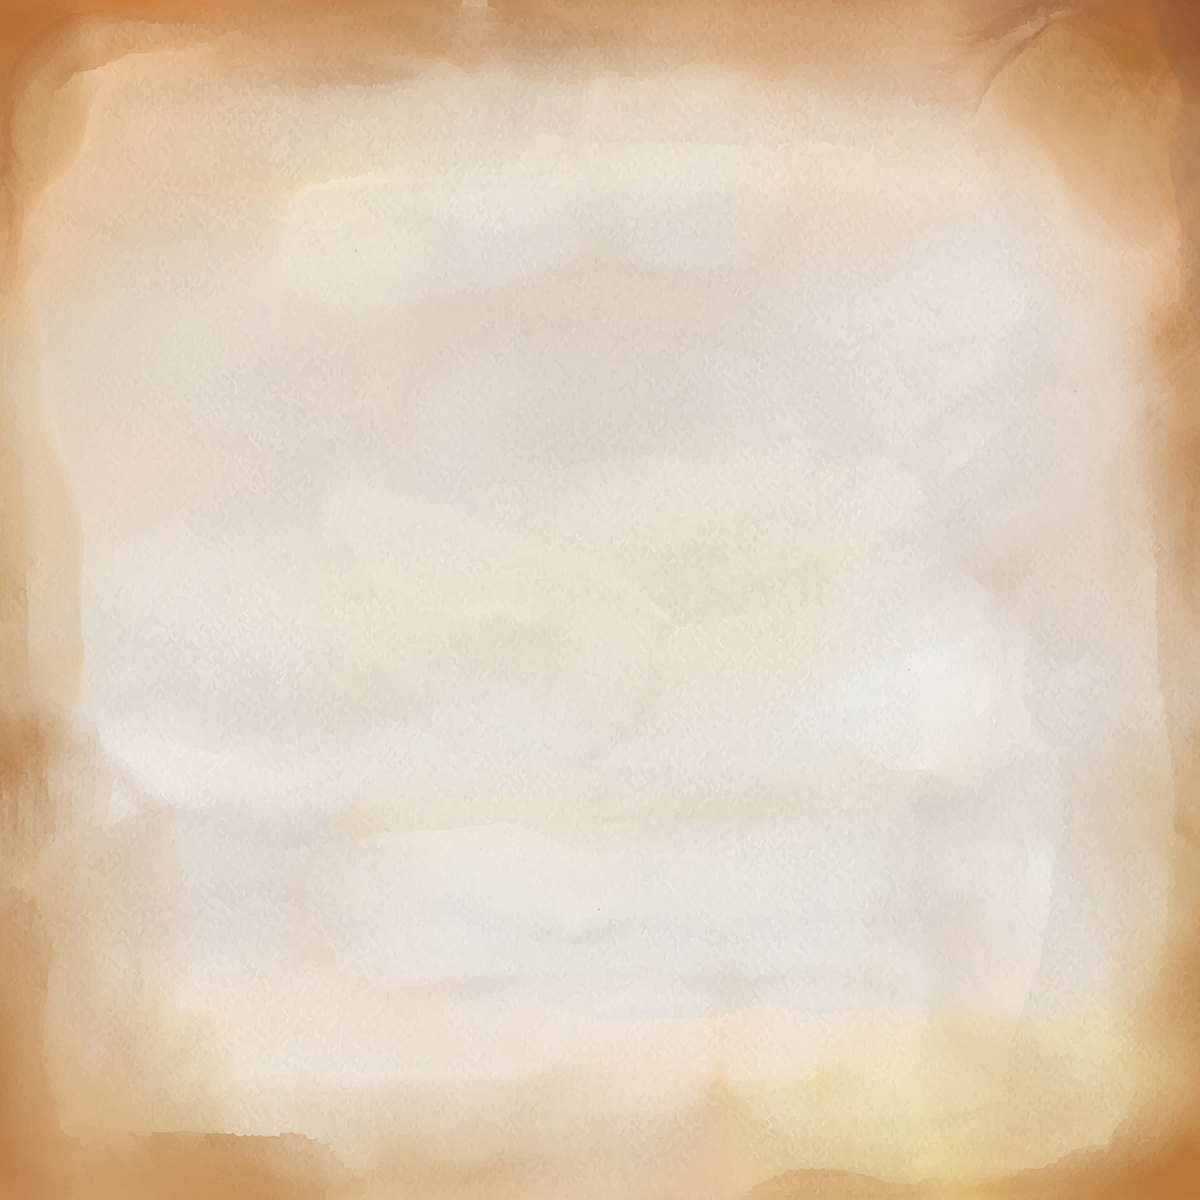
\includegraphics[keepaspectratio,% width=.9\textwidth,
      height=.8\textheight]{figures/old-paper-bg}
    };

    \node[text width=.8\textwidth, align=left, text justified, font=\itshape] at (0,0) {
      
      Karlsheim, 23 octobre de l’an 2514,\\

      Fiers aventuriers,\\

      Je vous écris sous les conseils avisés de maître Grimgoten, qui m’a
      conté vos récents exploits. Je suis le baron Erik Von Karl, chef d’une
      des plus anciennes familles nobles de la ville de Karlsheim.\\

      Depuis le début de l’automne, notre belle cité est en proie au
      terrible fléau de la peste. Il n’a suffit que d’un mois pour que des
      rues, qui autrefois étaient grouillantes de ferveur et de joie,
      laissent place à une atmosphère de souffrance et de mort. Un tiers de
      nos concitoyens ont d’ores et déjà été emportés par ce mal qui vous
      couvre de pustules et vous ronge de l’intérieur jusqu’à la folie.\\

      Les causes de l’apparition de la maladie sont pour moi évidentes: la
      récente ouverture de la frontière avec le Moot à des fins
      commerciales. Mes observateurs m’ont en effet fait remonter que
      plusieurs cas de peste avaient été déclarés chez les petites gens; ces
      mêmes petites gens avec qui nous commerçons.\\

      Il y a quelques jours de cela, le maire actuel de Karlsheim, Robert
      Verboten, voyant la situation lui échapper, a décrété le confinement
      de la ville. Ayant été appelé pour affaire à Nuln, je n’étais pas
      présent lorsque ce confinement a été décrété et vous écris donc depuis
      le camp dressé à l’extérieur de la cité.\\

      Au fur et à mesure des jours, les hurlements et les pleurs se sont
      fait entendre par delà les murailles de la ville. La panique s’est
      emparée de la population confinée j’en suis sur. Je ne peux
      qu'imaginer les horreurs que subissent mes concitoyens face à la
      maladie et aux privations. J’ai d’autant plus d’angoisse en sachant
      que ma fille, Rita Von Karl se trouve, en ce moment-même, seule dans
      la demeure Von Karl. La dernière fois que j’ai eu de ses nouvelles,
      elle était en parfaite santé. Qui c’est maintenant ce qu’il est advenu
      d’elle, alors que la maladie règne encore à l’intérieur des murs. \\

      Aventuriers, la chose que je m’apprête à vous demander n’est ni simple
      ni sans risque. Il s’agit de pénétrer dans Karlsheim, de trouver ma
      fille et de la ramener en lieu sûr. \\

      Rencontrons-nous dans mes quartiers du camp à l’entrée de la
      ville. Je pourrai alors vous en dire plus sur la mission, et sur la
      récompense.

      \begin{flushright}
        {\fontsize{14}{16}\selectfont{}E.Von Karl}
      \end{flushright}
    };
  \end{tikzpicture}

\end{figure}

\newpage

Le MJ doit lire le texte ci-dessous décrivant la situation de départ
des aventuriers.

\begin{mjbox}
  Votre groupe se dirige vers la ville de Karlsheim depuis le
  nord. Après avoir quitté les plaines du Stirland, vous pénétrez dans
  une forêt de hêtres, signe que les eaux du fleuve Stir sont à
  proximité. Vous avancez paisiblement, loin de vous douter des
  malheurs qui se trament à Karlsheim. A la nuit tombée, vous décidez
  de faire halte dans une clairière dont la sortie s’ouvre sur deux
  chemins. L’éveil nocturne de la forêt vous fait rester sur le
  qui-vive. Vos sens sont aux aguets pour déceler la moindre menace. A
  l’heure la plus noire de la nuit, votre sang ne fait qu’un tour car
  il vous semble distinguer au loin des râles de
  douleurs\dots \\

  Vous vous réveillez le lendemain avec le peu de sommeil qu’il vous
  a été donné de prendre. Les cendres du feu sont encore
  chaudes. Après une collation frugale, vous devez décider de la
  route à suivre pour vous rendre au campement à la rencontre d’EVK.
\end{mjbox}

Ici le MJ doit décrire aux PJs les deux chemins possibles pour arriver
au camp. Le premier s’oriente vers le sud-est et est un chemin
paisible vers Karlsheim. Le second, qui prend la direction du
sud-ouest, mène vers un petit mausolée en ruines. Au cas où les PJs
demandent à inspecter l’entrée des deux chemins, un test de Perception
réussi révélera la présence de nombreuses empreintes d’animaux partant
dans la direction opposée à celle du chemin menant au mausolée. Selon
le choix des PJs d’emprunter l’un ou l’autre chemin, deux scénarios
sont possibles:

\begin{enumerate}
\item Si les PJs choisissent le chemin du sud-est, ils arrivent
  paisiblement au camp de Karlsheim. Dans ce cas, passez directement
  à la partie \nameref{sec:arrivee-au-camp}.
\item Si les PJs choisissent le chemin du sud-ouest, ils s’aventurent
  jusqu’au mausolée en ruines. Dans ce cas là, lire
  \nameref{sec:mausolee}.
\end{enumerate}

\subsection{Le mausolée}
\label{sec:mausolee}

\begin{mjbox}
  Malgré tous les signes inquiétants qui semblaient vous dissuader
  d’emprunter ce chemin, vos pas vous conduisent à l’entrée d’un
  bâtiment en ruine. La mousse a peu à peu recouvert les pierres de
  taille mais cela n’enlève rien au caractère solennel et imposant de
  l’édifice. Les statues des gardiens du jardin de Morr qui entourent
  l’entrée vous font comprendre qu’il s’agit là d’un mausolée. Votre
  attention est attirée par l’état de la grille qui permet l’accès au
  tombeau. Celle-ci semble en effet avoir été forcée récemment.
\end{mjbox}

Si les PJs décident d’entrer dans le mausolée, ils rencontrent un
disciple de Nurgle (humain faisant partie d’une secte louant le dieu
du chaos Nurgle, seigneur de la pestilence et de la
maladie). Plusieurs mutations, résultat de l’influence du chaos, sont
visibles sur son corps (décider des mutations en vous référant à la
table des Mutations du chaos). Un combat s’engage entre le disciple et
les PJs. Lorsque le disciple n’a plus qu’un point de vie ou au premier
coup critique non-mortel, les PJs interrogent l’ennemi agonisant.

\begin{mjbox}
  (Rires compulsifs mêlant la souffrance à la folie) \\
  \og Réjouissez-vous, grand-père (Nurgle) vous prendra bientôt en son
  sein… Arghh… Son oeuvre s’étend déjà à toute cette maudite ville de
  Karlsheim… Arghh…  La pestilence que nous avons conçue vous
  consumera bientôt dans d’exquises boursouflures suintantes… Arghh,
  arghhhhh...\fg{}
\end{mjbox}

\begin{gamebox}[coltext=guardsmanred]
  +1 point quant à la compréhension de l'origine de la peste
\end{gamebox}

\begin{gamebox}[title={NIVEAU DE COMPRÉHENSION SUR
    L'ORIGINE DE LA PESTE},%
  before upper={\tcbtitle},%
  center title,%
  titlerule=0pt,%
  toptitle=5pt,%
  coltitle=guardsmanred,%
  colbacktitle=gameboxbgcolor,%
  fonttitle=\fontsize{13}{15}\bfseries\selectfont]
 
  Si les PJs arrivent à interroger le disciple de Nurgle, ils
  acquièrent des informations vis à vis de l’origine de la peste à
  Karlsheim. Tout au long de l’aventure, les PJs vont pouvoir
  accumuler des points de compréhension les menant peu à peu vers la
  vérité. Il y a en tout 5 points à collecter. SI les PJs arrivent à
  obtenir 3 points sur les 5, la vérité sur la situation leur est
  révélée au moment opportun, et influencera la résolution de
  l’histoire ainsi que la récompense obtenue. La collecte des points
  se fera en fonction des choix des PJs en réponse aux différents
  évènements de l’aventure. Chaque point de compréhension acquis sera
  annoncé explicitement par la mention suivante:

  {\begin{gamebox}[coltext=guardsmanred] $(+\vert{}-)X$ point(s) quant
      à la compréhension de l’origine de la peste
    \end{gamebox}}
\end{gamebox}

Par ailleurs, si les PJs décident de fouiller le cadavre du disciple,
ils découvrent une arbalète de poing de bonne qualité ainsi que 20
carreaux.

\subsection{L'arrivée au camp}
\label{sec:arrivee-au-camp}


\end{document}